\documentclass{article}
\usepackage{tikz}
\usetikzlibrary{positioning, arrows.meta, calc}

\begin{document}

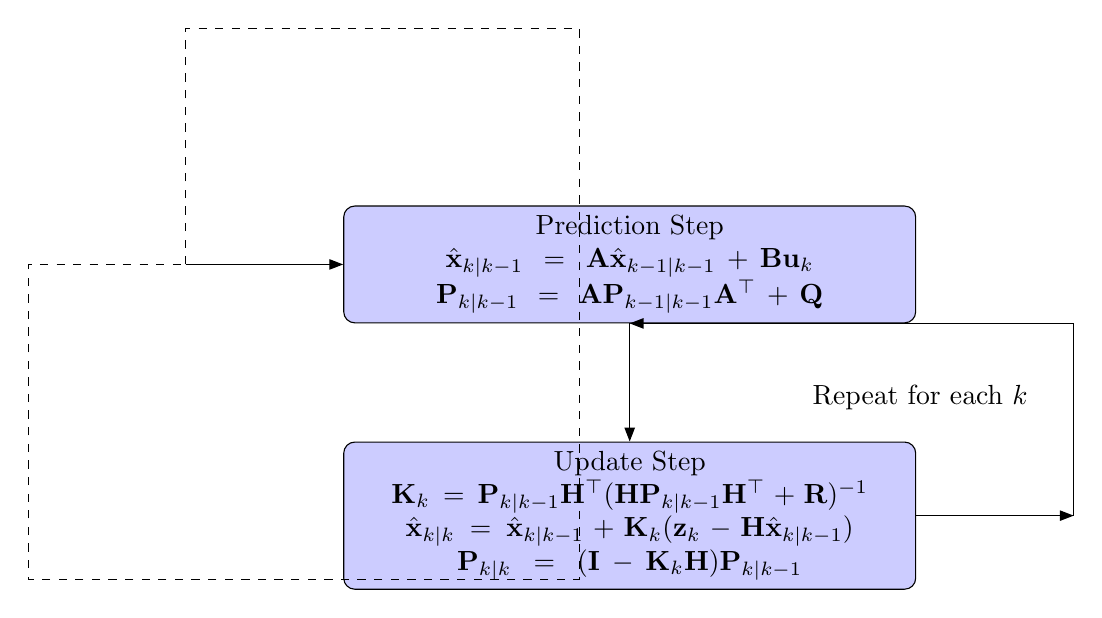
\begin{tikzpicture}[node distance=2cm, auto, >={Stealth[inset=0pt,length=5pt]}]
    % Styles
    \tikzstyle{block} = [rectangle, draw, fill=blue!20,
    text width=20em, text centered, rounded corners, minimum height=4em]
    \tikzstyle{input} = [coordinate]
    \tikzstyle{output} = [coordinate]

    % Nodes
    \node [block] (predict) {Prediction Step \\ \(\hat{\mathbf{x}}_{k|k-1} = \mathbf{A} \hat{\mathbf{x}}_{k-1|k-1} + \mathbf{B} \mathbf{u}_k\) \\ \(\mathbf{P}_{k|k-1} = \mathbf{A} \mathbf{P}_{k-1|k-1} \mathbf{A}^\top + \mathbf{Q}\)};
    \node [block, below=1.5cm of predict] (update) {Update Step \\ \(\mathbf{K}_k = \mathbf{P}_{k|k-1} \mathbf{H}^\top (\mathbf{H} \mathbf{P}_{k|k-1} \mathbf{H}^\top + \mathbf{R})^{-1}\) \\ \(\hat{\mathbf{x}}_{k|k} = \hat{\mathbf{x}}_{k|k-1} + \mathbf{K}_k (\mathbf{z}_k - \mathbf{H} \hat{\mathbf{x}}_{k|k-1})\) \\ \(\mathbf{P}_{k|k} = (\mathbf{I} - \mathbf{K}_k \mathbf{H}) \mathbf{P}_{k|k-1}\)};
    \node [input, left=2cm of predict] (init) {Initialization};
    \node [output, right=2cm of update] (output) {Output: \\ \(\hat{\mathbf{x}}_{k|k}\) and \\ \(\mathbf{P}_{k|k}\)};

    % Arrows
    \draw [->] (init) -- (predict);
    \draw [->] (predict) -- (update);
    \draw [->] (update) -- (output);
    \draw [->] (update.east) -- ++(2,0) |- (predict.south);

    % Draw boxes
    \draw[dashed] (init) -- ++(0,3) -- ++(5,0) -- ++(0,-7) -- ++(-7,0) -- ++(0,4) -- cycle;

    % Labels
    \node at ($(predict.north)!0.5!(update.south)+(2.2cm,0)$) [anchor=west] {Repeat for each \( k \)};
\end{tikzpicture}

\end{document}
